\documentclass{article}  
\usepackage{amsmath}
\usepackage{graphicx}
\usepackage{scrextend}
\usepackage[english]{babel}
\usepackage{blindtext}
\usepackage[margin=1in]{geometry}
\usepackage{setspace}
\renewcommand{\baselinestretch}{1.5}

\title{
CSCE578 Assignment 3 Report
}
\author{Sebastian Martin}
\begin{document}
\maketitle


\begin{addmargin}[4em]{4em}
The main objective of this project was to categorize multiple reddit forums into clusters to see how they overlap. In order to achieve this the online forum Reddit was used. Reddit is a website that allowed users to create small groups, or subreddits, that have a certain theme. In this situation political themes were chosen, such as Donald Trump $($r$/$the\_donald$)$ and Socialism $($r$/$socialism$)$. The reasons why these were chosen is because reddit is one of the most visited websites with over 500 million monthly visitors to the site. It is also a generally anonymized website that only requires an email to create an account so many people are willing to post strong opinions.
\\
The first step in this process was to create a developer account for reddit that would allow be to receive an API key and secret in order to have a large amount of API calls to the website. After this a package called "praw" was used in order to efficiently create the API calls to reddit and to parse the data into its parts. As the limit per Subreddit is 500, there was a limit to how many posts were able to be pulled down. In order to slightly combat this, only the most popular 500 posts from each Subreddit were analyzed. One this was done a simple .txt was created that held all of the data. \\
The actual data that was fed through the process at the end was a concatenation of the title of the post, and the body of the post. This was done in order to receive the greatest amount of text to process. Another issue was that Reddit, much like most social media is filled mostly with images and memes, which were not processed.
\\ 
Once all of the text had been found and cleaned it was able to be analyzed.
The method used to complete this was a TF-IDF (term frequency – inverse document frequency) computation on the post data. This was done in order to gain an insight into which words were the most important to each of the posts. After all of these had been done the data needed to be reduced in dimension to 2 for graphing and clustering.
\\
In order to achieve this process a t-SNE (T-distributed Stochastic Neighbor Embedding) statistical procedure was applied to the entire matrix of TF-IDF values to create 2 dimensional points for each of the documents$($posts$)$. Once this was completed it was simple to graph the data on a cartesian plane. Following this process a k$-$means clustering was applied to all of the points in order to group them in coherent clusters. To achieve this a cluster count of 9 was chosen because this is how many individual subreddits were scraped for the data, and hopefully they would have fallen back into their own respective clusters. 
\\
The results of this can be seen below:\\
\end{addmargin}

\begin{figure}[!h]
  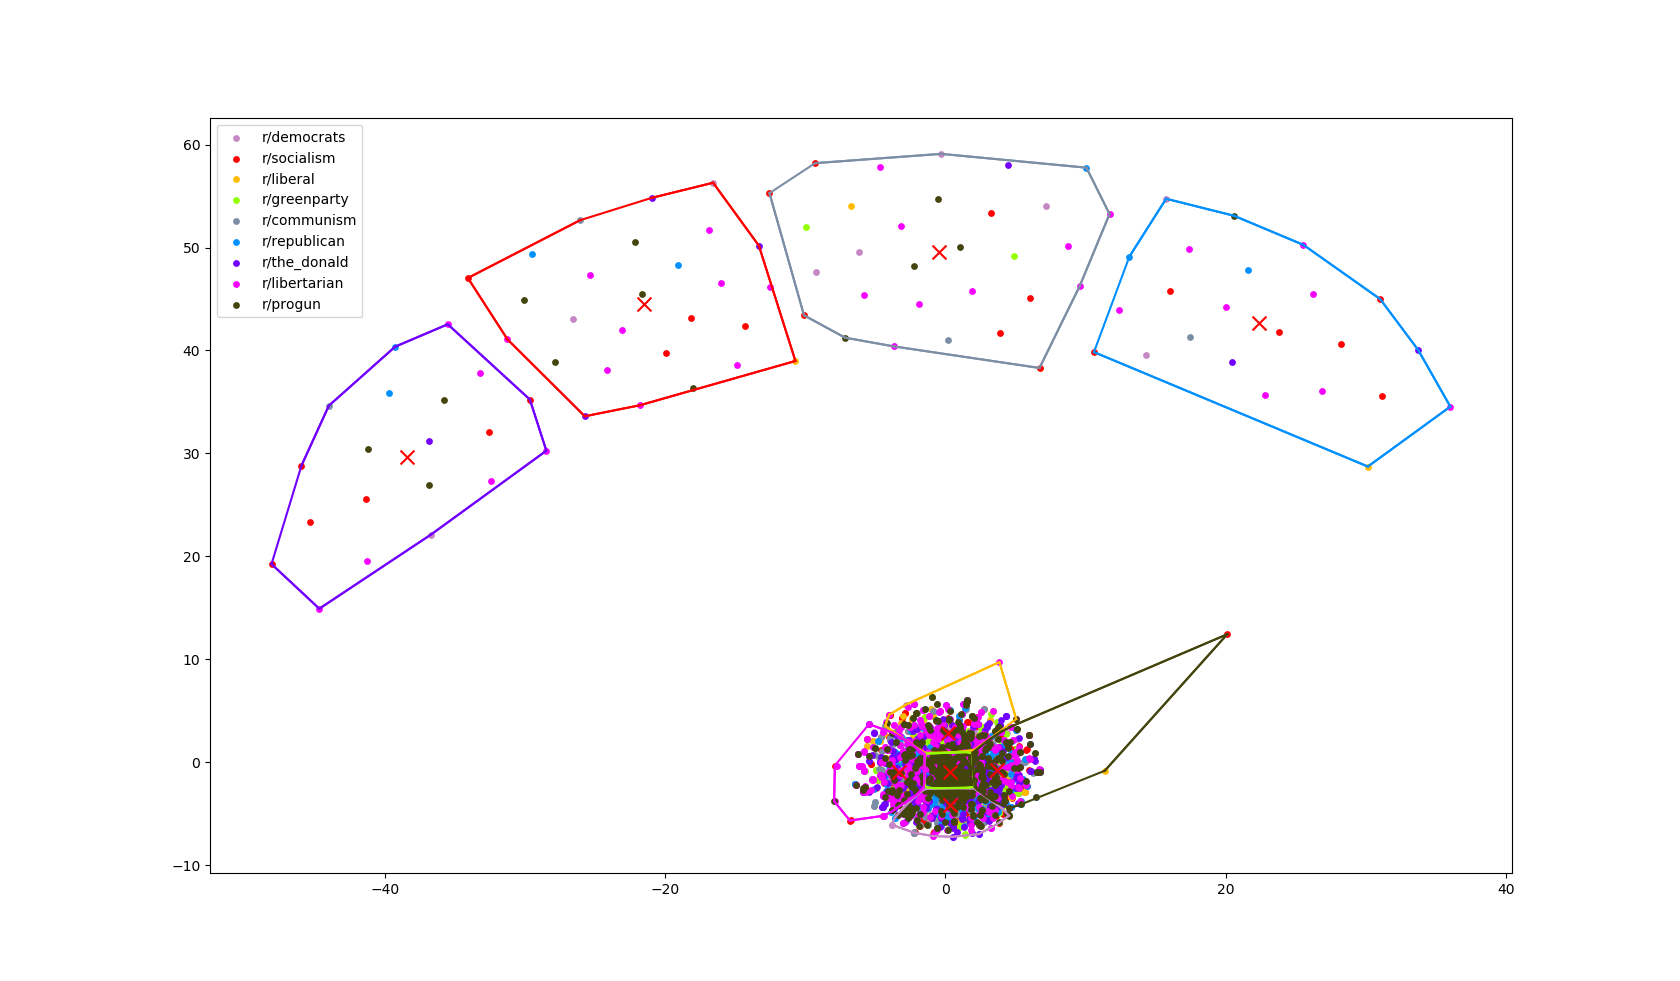
\includegraphics[width=\linewidth]{Figure_2.png}
  \caption{Scatter plot}
  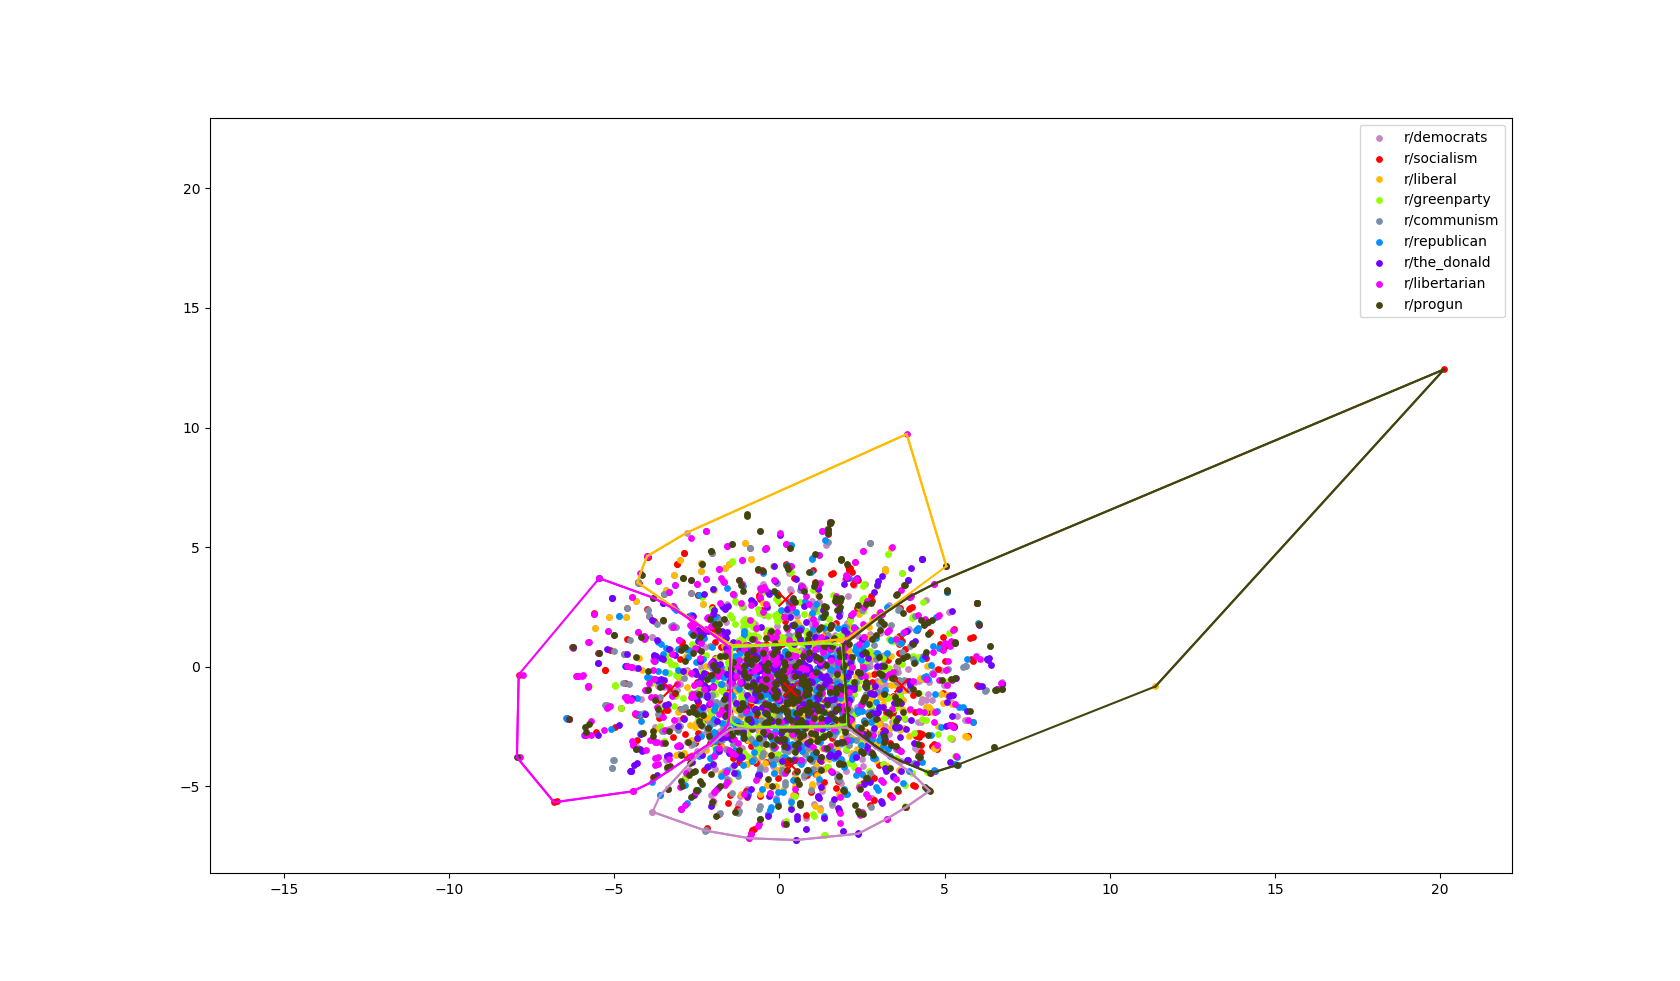
\includegraphics[width=\linewidth]{Figure_3.png}
  \caption{Zoomed Scatter plot}
  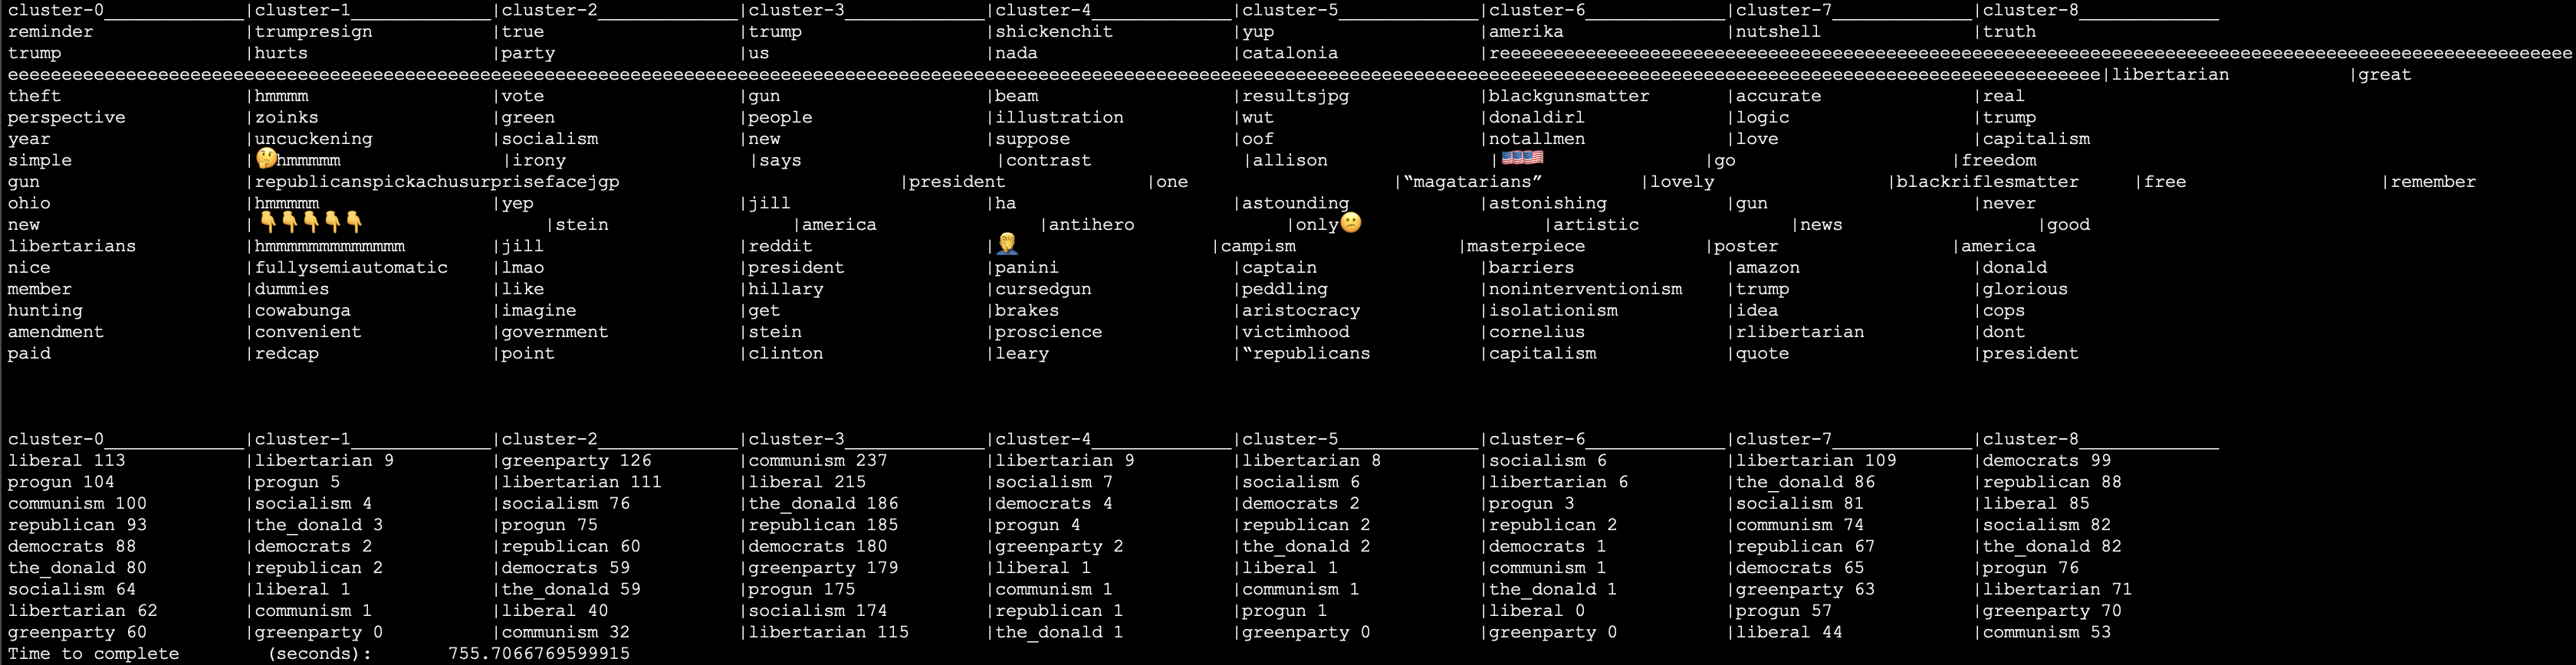
\includegraphics[width=\linewidth]{SS1.png}
  \caption{Zoomed Scatter plot}
\end{figure}
\begin{addmargin}[4em]{4em}
Looking at the above scatterplots it is obvious that nearly all of the ideologies overlap dramatically. There is an absolutely huge mass of points congregated around cluster 3 (green) in the center of the cluster. Looking at the output of the most common words this comes as no surprise as the most commonly used phrases in these posts are "trump", "us", "gun" , "people", "america", "hillary", etc. These are important to every single political ideology in the United States. Generally, this trend continues over most of the clusters, all of the top words are commonly used in order to push an ideology. This includes words such as "logic", " news", "vote", "perspective", and "truth".  \\
Nearly all of the subreddits were having conversations about the same topics. Trump, guns, voting, and Hillary Clinton are the key talking points for all of them. \\
Because of this the data was not as telling about the overlaps in political ideals as was originally expected. Because the most important topics to each political ideology is general the same, They just have differing opinions about them. Because of this all of the posts seemed to gravitate toward one another without as much separation as was originally expected. In the future this could be furthered by finding larger data sets and figuring out how to incorporate positive, or negative, connotations along with the themes into the tf-idf, k-means clustering. This would solve the issue of repeating themes, without being able to tell the beliefs about the themes.\\\\
Another analysis that was completed on this data was the most common 2-word, 3-word, and 4-word phrases in each Subreddit.\\
This gave a much clearer example about what each Subreddit spends their time talking about and what popular topics of conversation are.\\
Looking at this we can see that the democratic Subreddit is completely infatuated with twitter, both from trump, and democratic senators. The most common 2 word phrase on the entire subreddit is "on twitter", closely followed by "the president". These trends continue from the 2 word pairs up to the 4 word pairs on this Subreddit, with phrases such as "jeff merkley on twitter". These trends continue all of the way through the subreddits. Socialism is mostly taking about trump as well, with the most popular phrases "trump supporter", "trump supporter is arrested", and "make america great again". Donald Trump dominates the political conversation on 5 out of the 9 Subreddits that were searched through. The only 4 where he did not were the Green Party, Communism Progun, and Libertarian Subreddit. These 4 all had their own political agendas as the most popular discussion pieces. Most notable the green party had presidential candidate Jill Stein on the top of all 3 phrase lists (2/3/4 pair). And ProGun had only Gun advocacy phrases on their list. Not a single mention of a presidential candidate or a political figure. One of the most interesting results was under the "the\_donald" Subreddit where the most common 2 word phrase is "hate crime", with it appearing with a rate of 5.8\% per post in the entire Subreddit. With donald trump only appearing at a rate of 4.2\% per post.\\
If this were to be continued, then possibly a combination of both of these processes could be used in order to gain insight into the overlap of these political forums. However, with the time constraints the result is better than expected. Figuring out that nearly all of these forums focus on the same issues through the k-means clustering, and finding the most common phrases in each subreddit allowed us to adequately see the ideals behind each of these communities.

\end{addmargin}


What each file is:
\begin{addmargin}[4em]{4em}
redditScraper.py - This pulled all of the data from Reddit and formatted it.\\
Analysis.py - This performed the TF-IDF, t-SNE, and k-Means analysis\\
checkPairs.py - Performed the finding of pairs in each Community \\
data/* - all of the data that was pulled from Reddit\\
data50/* - test data for all of the code (only 50 posts from each community)\\
phrases.txt - the document containing all of the 2/3/4 word phrases and thir counts.
\end{addmargin}




\end{document}
